
%% bare_conf.tex
%% V1.3
%% 2007/01/11
%% by Michael Shell
%% See:
%% http://www.michaelshell.org/
%% for current contact information.
%%
%% This is a skeleton file demonstrating the use of IEEEtran.cls
%% (requires IEEEtran.cls version 1.7 or later) with an IEEE conference paper.
%%
%% Support sites:
%% http://www.michaelshell.org/tex/ieeetran/
%% http://www.ctan.org/tex-archive/macros/latex/contrib/IEEEtran/
%% and
%% http://www.ieee.org/

%%*************************************************************************
%% Legal Notice:
%% This code is offered as-is without any warranty either expressed or
%% implied; without even the implied warranty of MERCHANTABILITY or
%% FITNESS FOR A PARTICULAR PURPOSE! 
%% User assumes all risk.
%% In no event shall IEEE or any contributor to this code be liable for
%% any damages or losses, including, but not limited to, incidental,
%% consequential, or any other damages, resulting from the use or misuse
%% of any information contained here.
%%
%% All comments are the opinions of their respective authors and are not
%% necessarily endorsed by the IEEE.
%%
%% This work is distributed under the LaTeX Project Public License (LPPL)
%% ( http://www.latex-project.org/ ) version 1.3, and may be freely used,
%% distributed and modified. A copy of the LPPL, version 1.3, is included
%% in the base LaTeX documentation of all distributions of LaTeX released
%% 2003/12/01 or later.
%% Retain all contribution notices and credits.
%% ** Modified files should be clearly indicated as such, including  **
%% ** renaming them and changing author support contact information. **
%%
%% File list of work: IEEEtran.cls, IEEEtran_HOWTO.pdf, bare_adv.tex,
%%                    bare_conf.tex, bare_jrnl.tex, bare_jrnl_compsoc.tex
%%*************************************************************************

% *** Authors should verify (and, if needed, correct) their LaTeX system  ***
% *** with the testflow diagnostic prior to trusting their LaTeX platform ***
% *** with production work. IEEE's font choices can trigger bugs that do  ***
% *** not appear when using other class files.                            ***
% The testflow support page is at:
% http://www.michaelshell.org/tex/testflow/



% Note that the a4paper option is mainly intended so that authors in
% countries using A4 can easily print to A4 and see how their papers will
% look in print - the typesetting of the document will not typically be
% affected with changes in paper size (but the bottom and side margins will).
% Use the testflow package mentioned above to verify correct handling of
% both paper sizes by the user's LaTeX system.
%
% Also note that the "draftcls" or "draftclsnofoot", not "draft", option
% should be used if it is desired that the figures are to be displayed in
% draft mode.
%
\documentclass[conference]{IEEEtran}
% Add the compsoc option for Computer Society conferences.
%
% If IEEEtran.cls has not been installed into the LaTeX system files,
% manually specify the path to it like:
% \documentclass[conference]{../sty/IEEEtran}





% Some very useful LaTeX packages include:
% (uncomment the ones you want to load)


% *** MISC UTILITY PACKAGES ***
%
%\usepackage{ifpdf}
% Heiko Oberdiek's ifpdf.sty is very useful if you need conditional
% compilation based on whether the output is pdf or dvi.
% usage:
% \ifpdf
%   % pdf code
% \else
%   % dvi code
% \fi
% The latest version of ifpdf.sty can be obtained from:
% http://www.ctan.org/tex-archive/macros/latex/contrib/oberdiek/
% Also, note that IEEEtran.cls V1.7 and later provides a builtin
% \ifCLASSINFOpdf conditional that works the same way.
% When switching from latex to pdflatex and vice-versa, the compiler may
% have to be run twice to clear warning/error messages.






% *** CITATION PACKAGES ***
%
\usepackage{cite}
% cite.sty was written by Donald Arseneau
% V1.6 and later of IEEEtran pre-defines the format of the cite.sty package
% \cite{} output to follow that of IEEE. Loading the cite package will
% result in citation numbers being automatically sorted and properly
% "compressed/ranged". e.g., [1], [9], [2], [7], [5], [6] without using
% cite.sty will become [1], [2], [5]--[7], [9] using cite.sty. cite.sty's
% \cite will automatically add leading space, if needed. Use cite.sty's
% noadjust option (cite.sty V3.8 and later) if you want to turn this off.
% cite.sty is already installed on most LaTeX systems. Be sure and use
% version 4.0 (2003-05-27) and later if using hyperref.sty. cite.sty does
% not currently provide for hyperlinked citations.
% The latest version can be obtained at:
% http://www.ctan.org/tex-archive/macros/latex/contrib/cite/
% The documentation is contained in the cite.sty file itself.






% *** GRAPHICS RELATED PACKAGES ***
%
\ifCLASSINFOpdf
  \usepackage[pdftex]{graphicx}
  % declare the path(s) where your graphic files are
  \graphicspath{{../pdf/}{../jpeg/}{figures}}
  % and their extensions so you won't have to specify these with
  % every instance of \includegraphics
  \DeclareGraphicsExtensions{.pdf,.jpeg,.png}
\else
  % or other class option (dvipsone, dvipdf, if not using dvips). graphicx
  % will default to the driver specified in the system graphics.cfg if no
  % driver is specified.
  % \usepackage[dvips]{graphicx}
  % declare the path(s) where your graphic files are
  % \graphicspath{{../eps/}}
  % and their extensions so you won't have to specify these with
  % every instance of \includegraphics
  % \DeclareGraphicsExtensions{.eps}
\fi
% graphicx was written by David Carlisle and Sebastian Rahtz. It is
% required if you want graphics, photos, etc. graphicx.sty is already
% installed on most LaTeX systems. The latest version and documentation can
% be obtained at: 
% http://www.ctan.org/tex-archive/macros/latex/required/graphics/
% Another good source of documentation is "Using Imported Graphics in
% LaTeX2e" by Keith Reckdahl which can be found as epslatex.ps or
% epslatex.pdf at: http://www.ctan.org/tex-archive/info/
%
% latex, and pdflatex in dvi mode, support graphics in encapsulated
% postscript (.eps) format. pdflatex in pdf mode supports graphics
% in .pdf, .jpeg, .png and .mps (metapost) formats. Users should ensure
% that all non-photo figures use a vector format (.eps, .pdf, .mps) and
% not a bitmapped formats (.jpeg, .png). IEEE frowns on bitmapped formats
% which can result in "jaggedy"/blurry rendering of lines and letters as
% well as large increases in file sizes.
%
% You can find documentation about the pdfTeX application at:
% http://www.tug.org/applications/pdftex





% *** MATH PACKAGES ***
%
%\usepackage[cmex10]{amsmath}
% A popular package from the American Mathematical Society that provides
% many useful and powerful commands for dealing with mathematics. If using
% it, be sure to load this package with the cmex10 option to ensure that
% only type 1 fonts will utilized at all point sizes. Without this option,
% it is possible that some math symbols, particularly those within
% footnotes, will be rendered in bitmap form which will result in a
% document that can not be IEEE Xplore compliant!
%
% Also, note that the amsmath package sets \interdisplaylinepenalty to 10000
% thus preventing page breaks from occurring within multiline equations. Use:
%\interdisplaylinepenalty=2500
% after loading amsmath to restore such page breaks as IEEEtran.cls normally
% does. amsmath.sty is already installed on most LaTeX systems. The latest
% version and documentation can be obtained at:
% http://www.ctan.org/tex-archive/macros/latex/required/amslatex/math/





% *** SPECIALIZED LIST PACKAGES ***
%
%\usepackage{algorithmic}
% algorithmic.sty was written by Peter Williams and Rogerio Brito.
% This package provides an algorithmic environment fo describing algorithms.
% You can use the algorithmic environment in-text or within a figure
% environment to provide for a floating algorithm. Do NOT use the algorithm
% floating environment provided by algorithm.sty (by the same authors) or
% algorithm2e.sty (by Christophe Fiorio) as IEEE does not use dedicated
% algorithm float types and packages that provide these will not provide
% correct IEEE style captions. The latest version and documentation of
% algorithmic.sty can be obtained at:
% http://www.ctan.org/tex-archive/macros/latex/contrib/algorithms/
% There is also a support site at:
% http://algorithms.berlios.de/index.html
% Also of interest may be the (relatively newer and more customizable)
% algorithmicx.sty package by Szasz Janos:
% http://www.ctan.org/tex-archive/macros/latex/contrib/algorithmicx/




% *** ALIGNMENT PACKAGES ***
%
%\usepackage{array}
% Frank Mittelbach's and David Carlisle's array.sty patches and improves
% the standard LaTeX2e array and tabular environments to provide better
% appearance and additional user controls. As the default LaTeX2e table
% generation code is lacking to the point of almost being broken with
% respect to the quality of the end results, all users are strongly
% advised to use an enhanced (at the very least that provided by array.sty)
% set of table tools. array.sty is already installed on most systems. The
% latest version and documentation can be obtained at:
% http://www.ctan.org/tex-archive/macros/latex/required/tools/


%\usepackage{mdwmath}
%\usepackage{mdwtab}
% Also highly recommended is Mark Wooding's extremely powerful MDW tools,
% especially mdwmath.sty and mdwtab.sty which are used to format equations
% and tables, respectively. The MDWtools set is already installed on most
% LaTeX systems. The lastest version and documentation is available at:
% http://www.ctan.org/tex-archive/macros/latex/contrib/mdwtools/


% IEEEtran contains the IEEEeqnarray family of commands that can be used to
% generate multiline equations as well as matrices, tables, etc., of high
% quality.


%\usepackage{eqparbox}
% Also of notable interest is Scott Pakin's eqparbox package for creating
% (automatically sized) equal width boxes - aka "natural width parboxes".
% Available at:
% http://www.ctan.org/tex-archive/macros/latex/contrib/eqparbox/





% *** SUBFIGURE PACKAGES ***
%\usepackage[tight,footnotesize]{subfigure}
% subfigure.sty was written by Steven Douglas Cochran. This package makes it
% easy to put subfigures in your figures. e.g., "Figure 1a and 1b". For IEEE
% work, it is a good idea to load it with the tight package option to reduce
% the amount of white space around the subfigures. subfigure.sty is already
% installed on most LaTeX systems. The latest version and documentation can
% be obtained at:
% http://www.ctan.org/tex-archive/obsolete/macros/latex/contrib/subfigure/
% subfigure.sty has been superceeded by subfig.sty.



%\usepackage[caption=false]{caption}
%\usepackage[font=footnotesize]{subfig}
% subfig.sty, also written by Steven Douglas Cochran, is the modern
% replacement for subfigure.sty. However, subfig.sty requires and
% automatically loads Axel Sommerfeldt's caption.sty which will override
% IEEEtran.cls handling of captions and this will result in nonIEEE style
% figure/table captions. To prevent this problem, be sure and preload
% caption.sty with its "caption=false" package option. This is will preserve
% IEEEtran.cls handing of captions. Version 1.3 (2005/06/28) and later 
% (recommended due to many improvements over 1.2) of subfig.sty supports
% the caption=false option directly:
%\usepackage[caption=false,font=footnotesize]{subfig}
%
% The latest version and documentation can be obtained at:
% http://www.ctan.org/tex-archive/macros/latex/contrib/subfig/
% The latest version and documentation of caption.sty can be obtained at:
% http://www.ctan.org/tex-archive/macros/latex/contrib/caption/




% *** FLOAT PACKAGES ***
%
%\usepackage{fixltx2e}
% fixltx2e, the successor to the earlier fix2col.sty, was written by
% Frank Mittelbach and David Carlisle. This package corrects a few problems
% in the LaTeX2e kernel, the most notable of which is that in current
% LaTeX2e releases, the ordering of single and double column floats is not
% guaranteed to be preserved. Thus, an unpatched LaTeX2e can allow a
% single column figure to be placed prior to an earlier double column
% figure. The latest version and documentation can be found at:
% http://www.ctan.org/tex-archive/macros/latex/base/



%\usepackage{stfloats}
% stfloats.sty was written by Sigitas Tolusis. This package gives LaTeX2e
% the ability to do double column floats at the bottom of the page as well
% as the top. (e.g., "\begin{figure*}[!b]" is not normally possible in
% LaTeX2e). It also provides a command:
%\fnbelowfloat
% to enable the placement of footnotes below bottom floats (the standard
% LaTeX2e kernel puts them above bottom floats). This is an invasive package
% which rewrites many portions of the LaTeX2e float routines. It may not work
% with other packages that modify the LaTeX2e float routines. The latest
% version and documentation can be obtained at:
% http://www.ctan.org/tex-archive/macros/latex/contrib/sttools/
% Documentation is contained in the stfloats.sty comments as well as in the
% presfull.pdf file. Do not use the stfloats baselinefloat ability as IEEE
% does not allow \baselineskip to stretch. Authors submitting work to the
% IEEE should note that IEEE rarely uses double column equations and
% that authors should try to avoid such use. Do not be tempted to use the
% cuted.sty or midfloat.sty packages (also by Sigitas Tolusis) as IEEE does
% not format its papers in such ways.





% *** PDF, URL AND HYPERLINK PACKAGES ***
%
%\usepackage{url}
% url.sty was written by Donald Arseneau. It provides better support for
% handling and breaking URLs. url.sty is already installed on most LaTeX
% systems. The latest version can be obtained at:
% http://www.ctan.org/tex-archive/macros/latex/contrib/misc/
% Read the url.sty source comments for usage information. Basically,
% \url{my_url_here}.





% *** Do not adjust lengths that control margins, column widths, etc. ***
% *** Do not use packages that alter fonts (such as pslatex).         ***
% There should be no need to do such things with IEEEtran.cls V1.6 and later.
% (Unless specifically asked to do so by the journal or conference you plan
% to submit to, of course. )


% correct bad hyphenation here
\hyphenation{vis-ual lang-u-ages}


\begin{document}
%
% paper title
% can use linebreaks \\ within to get better formatting as desired
\title{Measuring the Programmatic Intricacy of App Inventor Projects Grouped by Functionality}


% author names and affiliations
% use a multiple column layout for up to three different
% affiliations
\author{\IEEEauthorblockN{Benjamin Xie, Isra Shabir, and Hal Abelson}
\IEEEauthorblockA{Department of Electrical Engineering and Computer Science\\
Massachusetts Institute of Technology\\
Cambridge, Massachusetts, USA\\
Email: \{bxie, ishabir, hal\}@mit.edu}}
%\and
%\IEEEauthorblockN{Isra Shabir}
%\IEEEauthorblockA{Department of Electrical Engineering\\and Computer Science\\
%Massachusetts Institute of Technology\\
%Cambridge, Massachusetts 02139\\
%Email: ishabir@mit.edu}
%\and
%\IEEEauthorblockN{James Kirk\\ and Montgomery Scott}
%\IEEEauthorblockA{Starfleet Academy\\
%San Francisco, California 96678-2391\\
%Telephone: (800) 555--1212\\
%Fax: (888) 555--1212}}

% conference papers do not typically use \thanks and this command
% is locked out in conference mode. If really needed, such as for
% the acknowledgment of grants, issue a \IEEEoverridecommandlockouts
% after \documentclass

% for over three affiliations, or if they all won't fit within the width
% of the page, use this alternative format:
% 
%\author{\IEEEauthorblockN{Michael Shell\IEEEauthorrefmark{1},
%Homer Simpson\IEEEauthorrefmark{2},
%James Kirk\IEEEauthorrefmark{3}, 
%Montgomery Scott\IEEEauthorrefmark{3} and
%Eldon Tyrell\IEEEauthorrefmark{4}}
%\IEEEauthorblockA{\IEEEauthorrefmark{1}School of Electrical and Computer Engineering\\
%Georgia Institute of Technology,
%Atlanta, Georgia 30332--0250\\ Email: see http://www.michaelshell.org/contact.html}
%\IEEEauthorblockA{\IEEEauthorrefmark{2}Twentieth Century Fox, Springfield, USA\\
%Email: homer@thesimpsons.com}
%\IEEEauthorblockA{\IEEEauthorrefmark{3}Starfleet Academy, San Francisco, California 96678-2391\\
%Telephone: (800) 555--1212, Fax: (888) 555--1212}
%\IEEEauthorblockA{\IEEEauthorrefmark{4}Tyrell Inc., 123 Replicant Street, Los Angeles, California 90210--4321}}




% use for special paper notices
%\IEEEspecialpapernotice{(Invited Paper)}




% make the title area
\maketitle


\begin{abstract}
%\boldmath
MIT App Inventor is a web service that enables users with little to no previous programming experience to create applications for mobile devices using a visual blocks language. We analyze a random sample of projects to better understand the capability of using App Inventor to create Android applications of varying functionality. We group projects of similar functionality and measure the programmatic intricacy of these groups using multiple metrics. Our results depict qualitative differences in the learnability of the App Inventor service to implement apps of particular functionality. Our discussion addresses these findings in the context of App Inventor's learning resources.
\end{abstract}
% IEEEtran.cls defaults to using nonbold math in the Abstract.
% This preserves the distinction between vectors and scalars. However,
% if the conference you are submitting to favors bold math in the abstract,
% then you can use LaTeX's standard command \boldmath at the very start
% of the abstract to achieve this. Many IEEE journals/conferences frown on
% math in the abstract anyway.

% no keywords




% For peer review papers, you can put extra information on the cover
% page as needed:
% \ifCLASSOPTIONpeerreview
% \begin{center} \bfseries EDICS Category: 3-BBND \end{center}
% \fi
%
% For peerreview papers, this IEEEtran command inserts a page break and
% creates the second title. It will be ignored for other modes.
\IEEEpeerreviewmaketitle



\section{Introduction}

% no \IEEEPARstart


% You must have at least 2 lines in the paragraph with the drop letter
% (should never be an issue)


%\hfill mds
 
%\hfill April 3, 2015

%\subsection{MIT App Inventor}
MIT App Inventor is an environment that leverages a blocks-based visual programming language to create mobile apps for Android devices. An App Inventor project consists of a set of components and a set of blocks which give the components functionality. Components include items seen on the app (e.g. buttons, text boxes, images, drawing canvas) as well as non-visible items (e.g. camera, accelerometer, speech recognizer, GPS location sensor). The app's functionality is programmed in Blockly, a visual blocks-based programming language. For example, Figure 1 shows blocks for an app to prevent texting while driving. When a text is received, a predefined message is sent back to the person who sent the original text.

\begin{figure}[h!]
	\centering
	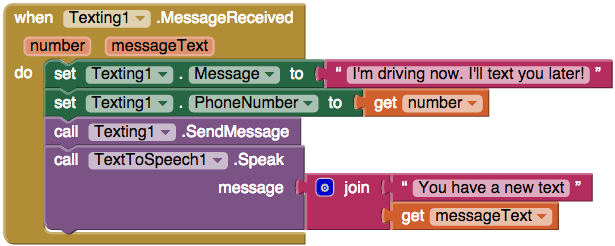
\includegraphics[width=0.95\linewidth]{fig1.png}
	\caption{Blocks for an App Inventor 2 project that automatically responds to texts received with a predefined message.}
	\label{FIgure 1: Label}
\end{figure}

There have been two major versions of App Inventor. App Inventor Classic (also known as App Inventor 1) was released in 2009 and ran the blocks editor from a separate Java application. In late 2013, App Inventor 2 (AI2) was released; the blocks editor now runs in a web browser as a Javascript program.\cite{naming:turbak} Although both versions of App Inventor are currently still in use, as of February 2015, 90\% of App Inventor users use App Inventor 2.\cite{ai_usage} For this reason, this research focuses on App Inventor 2 data.

App Inventor is taught at both grade school and college level, to a broad audience. Reports on courses taught depict App Inventor being used to create very diverse apps. These apps range from apps that discourage texting while driving to apps that track school buses to apps that organize community service cleanups.\cite{thinking:turbak} The pattern we see is that App Inventor enables "situated computing." This quarter-century old concept suggests that the convergence of computing, connectivity, and content enables users to use computing to bridge the gap between intentions and actions. App Inventor enables users to leverage their mobile devices to solve everyday problems they encounter. \cite{situated:hirakawa}

App Inventor also has copious resources for self-learners, typically in the form of self-contained tutorials. The App Inventor resources page includes 26 tutorials ranging from basic to intermediate to advanced difficulty. Most tutorials involve creating an entire functioning app from start to finish. Each tutorial typically focuses on either a new component or additional functionality for a previously introduced component.\cite{ai_tutorials}

To date, over 3.1 million users from 195 countries have created over 8.2 million apps with App Inventor. There are over 100,000 weekly active users.\cite{ai_home}

\subsection{Objective}
We seek to better understand what users create with App Inventor and determine what kinds of apps the App Inventor environment lends itself towards creating. We define metrics to measure the intricacy of the projects, measuring the proficiency of the blocks code used to program the apps. From this, we determine how easy it is to create an app of a certain functionality as well as the extent of capabilities App Inventor provides to implement certain functions. 

We analyze a random sample of projects and group them based on the components used in the app. To measure intricacy, we look at both the number of unique blocks in projects as well as the existence of more advanced programmatic structures, such as procedures, lists, and loops. From this, we evaluate how well suited App Inventor environment is to create apps with different functionalities and behaviors.

In this paper, we explain our technical approach to extracting information from raw project data, filtering and grouping projects, and comparing the intricacy of groups given our metrics.  We then discuss our findings in the context of the App Inventor service and its teaching resources.

\subsection{Previous Work}
Previously, analysis of App Inventor Classic has been done mostly at a user level.\cite{blocks:okerlund} Some of the notable findings include:
\begin{itemize}
	\item 30\% of projects have no blocks and therefore are not functional.
	\item Nearly 50\% of users do not have a single block or component in their projects.
	\item 53\% of users only have 1 project.
	\item A large number of procedures are only called 0 or 1 time.
\end{itemize}
This indicated that a large number of App Inventor Classic projects were never completed. It was theorized that a major contributing factor is the usability of the service. Whereas App inventor 2 is a single-page web service, App Inventor Classic required the deployment of an external Java service to program the app. This motivated the significant changes in the blocks language for App Inventor 2 to focus on usability.

\section{Technical Approach}

We extract features from a random sampling of App Inventor 2 projects. We group projects based on functionality by considering the components they contain and measure intricacy by the total number of unique blocks in the project as well as the existence of "multiplier" structures. We then look at each group and the distribution of the intricacy of projects in each group.

\subsection{Data Source}
Our source data is 5,228 random App Inventor 2 projects. We randomly selected projects according to their project ID, a sequentially increasing number (so a project with a lesser project ID corresponds to a project made earlier). The 5,228 projects selected come from 5,174 users, suggesting that randomization was accomplished. Given the size of the dataset and the randomness of the selection, we assume that the sample is representative of all App Inventor 2 projects. We use Pandas, a python data analysis library, for most of our data processing 

Of the 5,228 projects sampled...
\begin{itemize}
	\item At leasts 20\% (1,031 projects) are recreations of tutorials. These recreations of the step-by-step tutorials were found by matching project names. We only look at the 25 tutorials from the App Inventor website, although there exist many other tutorials made by other groups and individuals.\cite{ai_tutorials} These tutorials are included in our dataset.
	\item 16\% (845 projects) define procedures yet only 13\% (670 projects) call the procedures multiple times and use the procedures appropriately.	
\end{itemize}

We also find that 21\% (1,107 projects) are Certainly Non-Functional (CNF), or are guaranteed to be incomplete apps that have no behavior. If an app is without components, then there is nothing the user can interact with or for the app to do, so it cannot have functionality. In order for an app to have functionality, it must have at least two blocks: One to handle an event and one to respond to an event. Figure 2 shows an example of a simple action from two blocks. No functionality can occur with less than two blocks. We say an app is CNF if it either has no components or has fewer than two blocks.

\begin{figure}[h!]
	\centering
	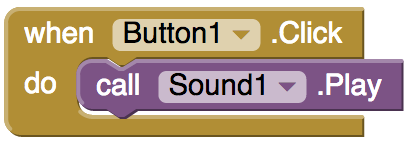
\includegraphics[width=0.55\linewidth]{simple_blocks.png}
	\caption{The simplest app behavior requires at least two blocks: An event handler and a resulting action. Here, a sound is played when a button is pressed.}
	\label{FIgure 2: Most Basic Block Example}
\end{figure}

\subsection{Feature Extraction}
We focus primarily on quantitative features to enable us to run clustering algorithms. In particular, we look at the number of each kind of component in a project, as well as the number of each type of block. The type of a component or block is provided in the source code of the project. 

Features Extracted from Projects:
\begin{itemize}
	\item Project Name
	\item User Name (anonymized)
	\item Number of Screens in Project
	\item Number of Components by Type
	\item Number of Blocks by Type
\end{itemize}

\subsection{Grouping Projects}
We group projects according to the components they contain. The palette in App Inventor organizes components by functionality and places each group in its own "drawer". Because the palette neatly organizes components into drawers of similar functions, we use it to define our groups. (Figure 3). 

\begin{figure}[h!]
	\centering
	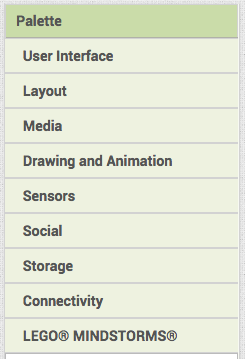
\includegraphics[width=0.4\linewidth]{palette.png}
	\caption{The palette in App Inventor 2 groups components into categories. These categories are used to group projects by functionality.}
	\label{FIgure 3: AI Designer Palette}
\end{figure}

We follow the palette drawers to define our groups, with two notable changes: Disregarding the "Layout" component drawer entirely as well as the sound and clock/timer components in our consideration of functionality groups. 

Layout components were removed as they are extraneous and irrelevant when grouping by functionality. Layout components enable users to change the visual display of apps and nothing further. Since we group projects by their functionality and layout components add no additional behavior to apps, they are disregarded.

The sound and clock components were removed to improve the differentiation between groups without detracting from the purpose of the app. The sound component (media drawer) plays a sound whenever the user specifies. Examples include playing a "meow" when an image of a cat is pressed to playing a famous speech in a historical quiz app. The clock (sensor) component enables apps to keep track of time. Uses for this are varied, ranging from keeping time in a stopwatch app to keeping time to periodically moving a sprite in a game app. The components certainly offer functionality to apps, but the component alone gives little affordance as to the intended behavior of the app. Because the sound and clock/timer components have very general uses and are often used, they do not help differentiate groups and are also excluded in the consideration of functionality groups.

There are eight groups. Basic apps only contain User Interface components (and possible Layout components, but they are ignored). \emph{Media}, Drawing, Sensor, Social, Storage, Connectivity, and Lego contain at least one component in the respective group in the palette. This categorization allows for overlap, as projects that contain components from multiple palette groups may be placed into multiple groups. In example, a project that uses both bluetooth (connectivity) and  twitter (social) component would be labelled both Connectivity and Social. The exception is the Lego group, which we deemed to be an exclusive group because of the specificity of the components. Since Lego components are solely for integration with Lego Mindstorms, they produce the most specific apps. So if a project contains a Lego component, it is grouped as only Lego, regardless of other components it may contain. 

Reiterating, Basic and Lego groups are disjoint from other groups and each other. Other groups may overlap. Table 1 provides a description of each group, the condition for a project to be in that group, and example components from that group.

\begin{table}[h!]
% increase table row spacing, adjust to taste
\renewcommand{\arraystretch}{1.3}
% if using array.sty, it might be a good idea to tweak the value of
% \extrarowheight as needed to properly center the text within the cells
\caption{Functionality Groupings}
\label{table_groups}
\centering
% Some packages, such as MDW tools, offer better commands for making tables
% than the plain LaTeX2e tabular which is used here.
%\begin{tabular}{ c | c | | c | c}
\begin{tabular}{| p{0.1\linewidth} | p{0.25\linewidth} | p{0.25\linewidth} | p{0.2\linewidth} | }
\hline

Group Name &  Description of App Functionality & Condition & Example Components\\
\hline
\hline
Basic & Only basic user interface components and nothing further &Only User Interface Components & Button, Image, Label, Notifier, Textbox \\
\hline

Media & Playing/recording of audio or video & At least 1 media component (excluding "sound") &Camera, TextToSpeech, VideoPlayer \\
\hline

Drawing
&Use screen as canvas for drawing
&At least 1 drawing component
&Canvas, Ball, ImageSprite\\
\hline

Sensor
&Response to phones' sensors
&At least 1 sensor component (excluding "clock')
&Accelerometer Sensor, LocationSensor, NearField (NFC)\\
\hline


Social
&Communication via phone or web
&At least 1 social component
&Texting, Twitter, PhoneCall\\
\hline

Storage
&Saving information
&At least 1 storage component
&TinyDB, FusiontablesControl, File\\
\hline

Connect
&Networking with other apps and phones
&At least 1 connectivity component
&ActivityStarter, BluetoothClient, Web\\

\hline
Lego
&Control Lego Mindstorm kits
&At least 1 lego components
&NxtDrive, NxtLightSensor\\
\hline

\end{tabular}
\end{table}

While we used components to group projects, we use the blocks that provide components functionality to measure project intricacy.

\subsection{Measuring Programmatic Complexity}

We define the "intricacy" of an App Inventor project as a measurement of the proficiency and quality of the implementation, as evidenced by the blocks used to program it. Intricate projects tend to exhibit good coding practices, such as code reuse through procedures and loops. They also tend to use advanced structures such as lists. A more intricate app tends to either implement more complex components or uses components in a more advanced manner. 

Of particular focus in our measure of intricacy is code reuse. In example, consider the case where two functionally similar projects exist and Project A copies the same code in three locations whereas Project B defines a procedure and calls the procedure three times. We argue Project B exhibits strong coding practices as it leverages code reuse in the form of procedures and therefore is a more intricate project. Project A has a greater number of blocks, but Project B has a slightly greater number of unique blocks with the blocks to initialize and call a procedure. A project that appropriately uses a procedure or for-loop rather than copies and pastes blocks (creating redundant code) would show evidence of greater intricacy, even if the resulting app in either case has identical functionality. We define the procedure, loop, and list blocks to be multiplier structures, as they increase the intricacy by "multiplying" the functionality of the the blocks contained in the procedure, loop, or list.

We define two metrics for programmatic intricacy in App Inventor: The number of unique blocks and the existence of different multiplier structures in the blocks code. We choose the number of unique blocks instead of the total number of blocks so the measure of intricacy is not affected by redundant code. We check projects for the existence of multiplier structures to account for advanced constructs that suggest more intricate code. 

Note that we try to ensure that the constructs are used properly. In example, a project is only considered to have a procedure if it is not only initialized, but also called multiple times as procedures are supposed to be. A full description of the conditions to have a multiplier structure counted in a project is shown in Table 2.

\begin{table}[h!]
% increase table row spacing, adjust to taste
\renewcommand{\arraystretch}{1.3}
% if using array.sty, it might be a good idea to tweak the value of
% \extrarowheight as needed to properly center the text within the cells
\caption{Multiplier Structures}
\label{table_multiplier}
\centering
% Some packages, such as MDW tools, offer better commands for making tables
% than the plain LaTeX2e tabular which is used here.
%\begin{tabular}{ c | c | | c | c}
\begin{tabular}{| p{0.15\linewidth} | p{0.65\linewidth} | }
\hline
Structure & Condition \\
\hline \hline
Procedure & At least one procedure initialized and called multiple times\\
\hline
Loop & At least one loop block created\\ 
\hline
List & At least one list initialized\\
\hline

\end{tabular}
\end{table}

Our two metrics of the number of unique blocks and the existence of advanced, multiplier structures specifically addresses the issue of redundant coding when measuring the intricacy of a project's implementation.

\section{Results}
We group the projects by functionality and show the distribution. Next, we show the distribution of the number of unique blocks in projects for each group. Finally, we show the fraction of projects within each group that use certain multiplier structures.

\subsection{Grouping}
After grouping projects by functionality, we find that 77.3\% of projects can be categorized into exactly one group. The remaining projects were categorized across multiple groups. The 4,121 projects resulted in 5,369 categorizations into groups; on average, a project fits into 1.3 groups.

Due to simplicity and the availability of learning resources, the largest groups are the Basic and Drawing groups, each containing around 24\% of the projects. Since basic apps are simple to create as they only include user interface components, it follows that there is a large amount of them. And when looking at the App Inventor tutorials, we see that over half of the beginner tutorials most users start with involve the creation of a drawing app. So, this suggests that the large amount drawing apps users create are in the form of tutorials and projects that extend from tutorials.

The Lego group is the smallest, containing only 28 (0.5\%) projects. One likely reason is because there is an additional hardware requirement in the form of Lego Mindstorm kits to use an app grouped as Lego. Another is that there exists no official tutorial for Lego projects. The full breakdown is shown in Figure 4.

\begin{figure}[h!]
	\centering
	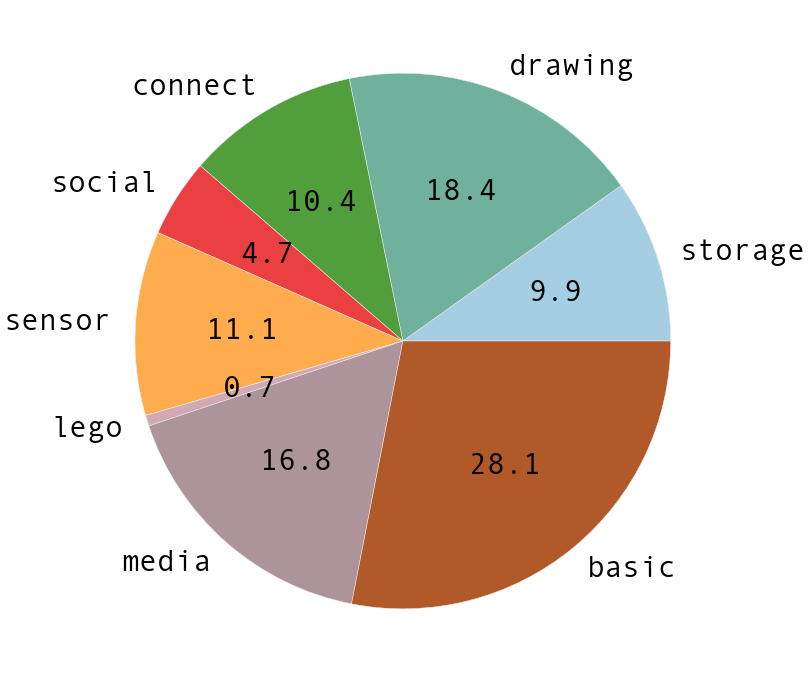
\includegraphics[width=0.9\linewidth]{pie_group.png}
	\caption{Functionality Groups by Size. 77.3\% of projects are categorized into exactly one group, with the others categorized across multiple groups}
	\label{Distribution of Groups}
\end{figure}

\subsection{Number of Unique Blocks}
We plot the distribution of the number of unique blocks in each group and compare these subsets of projects to each other and the entire set of projects.

Each subset and the entire set of projects exhibits a right skew, suggesting that each group contains a few outlier projects that have a significantly greater number of unique blocks and are likely well-developed projects.

Storage apps have the greatest median number of unique blocks, the widest distribution, and contains the project with the most number of unique blocks, suggesting that it has the greatest capability to create intricate apps.

The short distribution of the Lego group suggests its capabilities are limited. Despite this narrow distribution, it has a wide lower quartile (lower whisker). This wide lower quartiles suggests that even a simple project involving Lego components require more unique blocks to create. Developing these projects is not as intuitive and therefore more difficult to create.

Figure 5 and accompanying Table 3 shows the plot of the number of unique blocks of projects within each group, as well as the distribution for all projects ("All" in Figure 5). We reiterate that 23\% of projects fit into multiple groups, so one project can be represented in multiple plots. This is most evident in the outliers. In example, the greatest outlier is a password keeper app with 56 unique blocks in it; it is categorized as a Storage, Connect, and Media app because it has components of each of those types.

\begin{figure}[h!]
	\centering
	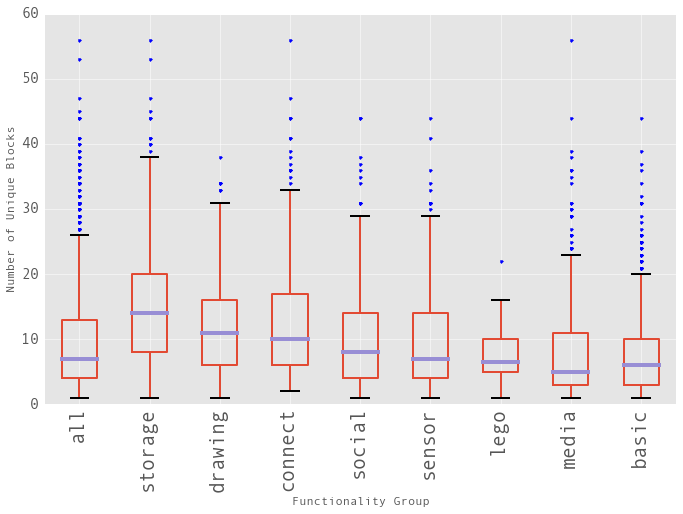
\includegraphics[width=1\linewidth]{boxplot.png}
	\caption{Distribution of Number of Unique Blocks by Functionality Group}
	\label{Distribution of Num of Unique Blocks}
\end{figure}

\begin{table}[h!]
% increase table row spacing, adjust to taste
\renewcommand{\arraystretch}{1.3}
% if using array.sty, it might be a good idea to tweak the value of
% \extrarowheight as needed to properly center the text within the cells
\caption{Summary Statistics for the Number of Unique Blocks by Group}
\label{table_noub_stats}
\centering
% Some packages, such as MDW tools, offer better commands for making tables
% than the plain LaTeX2e tabular which is used here.
%\begin{tabular}{ c | c | | c | c}
\begin{tabular}{| p{0.05\linewidth} | p{0.065\linewidth} | p{0.065\linewidth} | p{0.065\linewidth} | p{0.065\linewidth} | p{0.065\linewidth} | p{0.065\linewidth} | p{0.065\linewidth} | p{0.065\linewidth} | }
\hline

&basic
&lego
&media
&storage
&connect
&social
&sensor
&draw\\
\hline \hline


mean&
7.30&
7.86&
7.71&
15.39&
12.39&
10.12&
8.86&
10.67\\
\hline
std. dev.&
5.71&
4.86&
6.47&
9.27&
8.53&
8.62&
6.91&
6.39\\
\hline

min&
1&
1&
1&
1&
2&
1&
1&
1\\
\hline

max&
44&
22&
56&
56&
56&
44&
44&
38\\


\hline

\end{tabular}
\end{table}

\subsection{Multiplier Structures}
To visualize the existence of multiplier structures in each group, we plot the proportion of projects within each group that use procedures, loops, and lists. The results are depicted in Figure 6.

When looking at all projects across all groups ("All" in Figure 6), we see that the proportion of projects that use procedures and the proportion that use lists are approximately equal; the proportion of projects that use loops is about half compared to the other two. This relationship between proportion of multiplier structures does not hold true across all groups, suggesting that some multiplier structures are better suited for certain groups. We argue that the use of the loop and list structures vary by functionality of the app and therefore by group, but procedures tend to be more general in purpose.

Projects involving storage heavily use lists as temporary storage before moving information to a database or table as most projects categorized as storage tend to do. 

Drawing, Sensor, and Media apps' functionalities tend not to require the use of loops. Drawing apps often involve a user interacting with a canvas, such as using their finger to draw a picture. Sensor apps often respond to a sensor on the phone, such as responding to the shaking of the phone. Media apps often involve the recording or playing of audio or video. All three groups' functionalities often do not require iterating, so the proportion of loops evident in those groups is lower.

Because procedures only organize blocks and enable other blocks to be called easily, we argue its use is more general across groups. Whereas lists and loops perform a specific function, the functionality of a procedure is defined by the user and is therefore more general. We explore this further in the Discussion section. 

It is of note that the proportion of procedures existing in the Drawing group is abnormally high. Tutorials may in part explain this, as some popular beginning tutorials involve procedures, such as a "Whack-a-Mole" tutorial that uses a procedure to randomly move the mole the user is trying to whack. Users creating apps similar to these tutorials that contain procedures may only use the procedure in the manner described in the tutorial.

\begin{figure}[h!]
	\centering
	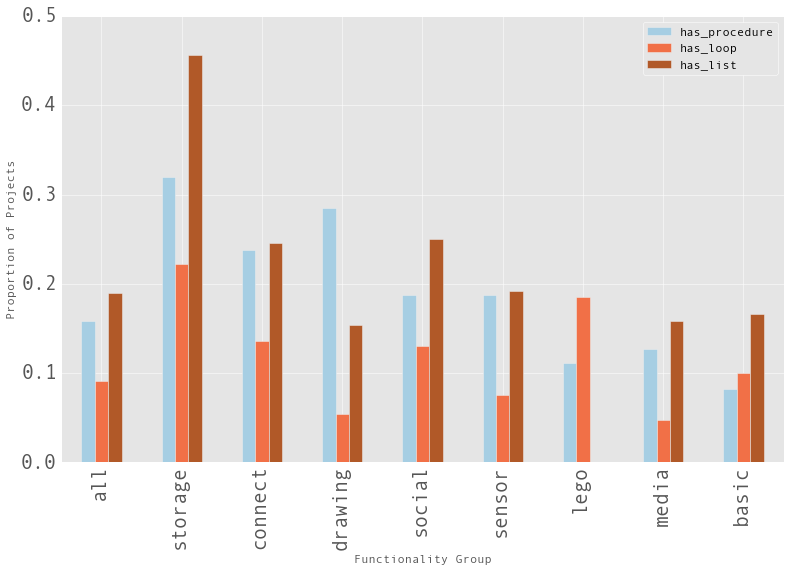
\includegraphics[width=1\linewidth]{multipliers.png}
	\caption{Proportion of Multiplier Structures by Functionality Group}
	\label{multipliers}
\end{figure}

\section{Discussion}
We critique our metrics of measuring intricacy and go on to analyze the intuitiveness of App Inventor to create different types of apps. We then tie this discussion on learnability back to App Inventor tutorials.

\subsection{Analysis of Metric}
When measuring the intricacy of projects, our challenge is in ensuring that the groups we categorize our projects in do not bias our metrics. That is, certain apps do not have greater or lesser intricacy just because they are in a certain group and perform a certain functionality. We argue that our metrics for the number of unique blocks and the proportion of projects in a group with procedures are our best metrics.

Because App Inventor features component-specific blocks, the number of unique blocks in a project is not directly dependent on its functionality. App inventor is event-driven, meaning the programming of App Inventor involves responding to an action, or event, relating to a component. This is made easy in App Inventor as each component has its own unique blocks to handle events, get and set attributes of the component, and call component functions. In Figure 7, we see that the button component has a block to handle it being pressed, the sound component has a block to play the sound, and the canvas has a block to change its color. Because App Inventor features blocks unique to each component, using one component instead of another does not inherently change the number of unique blocks in a project.

\begin{figure}[h!]
	\centering
	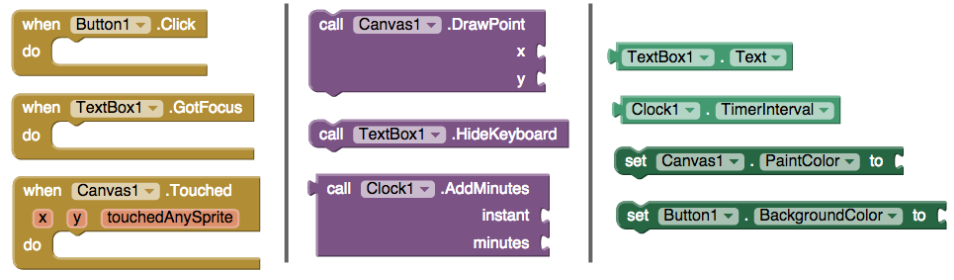
\includegraphics[width=1\linewidth]{component_blocks.png}
	\caption{Component-Specific Blocks. App Inventor features blocks that responding to events, getting/setting attributes, and component actions. For this reason, the number of unique blocks in a project is a suitable metric.}
	\label{component_specific_blocks}
\end{figure}

Whereas the proportion of loops and proportion of lists in projects can vary greatly depending on the functionality of it, the use of procedures are inherently not dependent on a certain functionality of the app. As mentioned in the results of the multiplier structures, we find that some functionalities rely more heavily on lists and loops than others. In example, drawing apps often have no use for loops but often use procedures to build reusable actions, such as erasing a drawing or resetting the score to a game. But the use of procedures is not dependent on functionality, as a procedure repeats whatever action the users defines when they create the procedure.

Because the number of unique blocks and proportion of projects with procedures do not depend on the functionality of projects, we focus primarily on these metrics in our analysis.

\subsection{Learnability}
A group is said to have high learnability if it does not require many different blocks to create a project. And if a group has high learnability, we expect many projects to be categorized into that group. We define a "learnability score" of a group as the ratio of the number of projects in the group divided by the the mean intricacy in Figure 8.  We argue that the learnability score is influenced by the beginner tutorials.

\begin{figure}[h!]
	\centering
	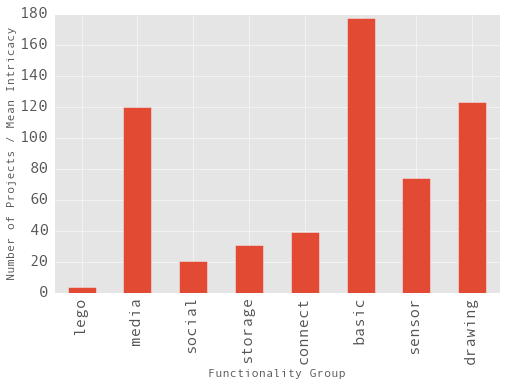
\includegraphics[width=1\linewidth]{learnability_score.png}
	\caption{Ratio of the Number of projects to mean intricacy, showing learnability of each group.}
	\label{LearnabilityScore}
\end{figure}

It is not surprising that Basic apps have the greatest learnability score and are therefore the easiest to learn. This follows since we define the Basic group as only containing user interface components and no other types of components. The Drawing and Media groups also have high learnability scores. This is likely because the tutorials introduced earlier on create Drawing apps and Media apps. The linear nature of App Inventor's tutorials causes the learnability score to follow closely with the sequence of tutorials.

The close correlation with learning scores and the sequence of tutorials suggests that users build off of knowledge from only the tutorials they complete. On the App Inventor website, tutorials are displayed in linear order and have levels ranging from "Basic" to "Intermediate" to "Advanced".\cite{ai_tutorials} Table 4 shows what functionality groups tutorials fit into. Most users tend to start at the basic tutorials but the number of tutorials made until users creates their own original projects varies. It is safe to assume that the earlier a tutorial appears in this sequence, the more users will use it. We see Drawing, Media and Sensor apps appear as basic tutorials; they are also have the highest learnability score. There are no Lego apps, and the very low learnability score reflects that. And although there are several tutorials involving storage, they appear under the advanced section. The lower learnability score suggests both that these later tutorials are viewed less and that storage apps are more intricate.

\begin{table}[h!]
% increase table row spacing, adjust to taste
\renewcommand{\arraystretch}{1.3}
% if using array.sty, it might be a good idea to tweak the value of
% \extrarowheight as needed to properly center the text within the cells
\caption{Grouping of App Inventor Tutorials}
\label{table_tutorial_group}
\centering
% Some packages, such as MDW tools, offer better commands for making tables
% than the plain LaTeX2e tabular which is used here.
%\begin{tabular}{ c | c | | c | c}
\begin{tabular}{| p{0.15\linewidth} | p{0.65\linewidth} | }
\hline

Level&
Functional Groups\\
\hline \hline
Basic&
Drawing(4), Media(2), Sensor(2), Basic\\
\hline 
Intermediate&
Drawing(5), Media(3), Storage, Social, Connect, Basic\\
\hline
Advanced&
Storage(5), Sensor(4), Connect(2), Drawing(2)\\

\hline

\end{tabular}
\end{table}

From our learnability score, we see that users tend to build off of the knowledge they gain from tutorials found earlier. This suggests that from the tutorials, users learn to create a specific type of app but not enough for this knowledge to generalize to create apps of other types with App Inventor. This can be seen as both a need for more generalizable tutorials and evidence of the vast capabilities of App Inventor to develop apps with broad functionality.


%%%%%%%%%%


\section{Conclusion}
We show that the number of unique blocks in a project as well as the proportion of projects that effectively use procedures both serve as sufficient measures of intricacy in the implementation of projects. By looking at the distribution of the number of unique blocks in projects of different groups, we are able to measure the capabilities for App inventor to develop apps of different functionalities. Our learning scores show that the learnability of specific functionalities of App Inventor closely relates to the functionalities in the basic, more popular tutorials. This suggests the amount of tutorials users complete are insufficient to provide them with enough generalizable knowledge of App Inventor to create original projects that are dissimilar from the tutorials they created.

We argue that breaking the sequentiality of the tutorials will better prepare users to deviate from tutorials and create more original apps. While we recognize that some functionality of App Inventor may inherently be more challenging than others, tutorials should still introduce more diverse components in the basic tutorials. The tutorials should also be displayed in such a way where users have a choice as to what to start with. We reiterate that our analysis is limited to the tutorials created by the MIT App Inventor team; the tutorials and curriculums made by other groups and individuals are out of the scope of this paper.

The existence of non-functional projects and recreations of tutorials in our dataset offer opportunities for future work. While we filtered out projects that were certainly non-functional by ensuring all projects had the minimum number of components and blocks, there still exist projects that do not have any functionality. Disregarding blocks that are not connected to other blocks and components with no programmed functionality would better filter out the non-functional projects. And while our findings suggest that the learnability score closely follows earlier tutorials, at least 20\% of the projects analyzed are recreations of the tutorials. Analyzing projects that are truly original would result in more robust findings. 

\section*{Acknowledgments}

This research is funded by the MIT EECS - Google Research and Innovation Scholarship. 

We thank Jeffery Schiller (MIT App Inventor) for help collecting the data and Ilaria Liccardi (MIT) and Franklyn Turbak (Wellesley College) for helping guide the analysis.


% trigger a \newpage just before the given reference
% number - used to balance the columns on the last page
% adjust value as needed - may need to be readjusted if
% the document is modified later
%\IEEEtriggeratref{8}
% The "triggered" command can be changed if desired:
%\IEEEtriggercmd{\enlargethispage{-5in}}

% references section

% can use a bibliography generated by BibTeX as a .bbl file
% BibTeX documentation can be easily obtained at:
% http://www.ctan.org/tex-archive/biblio/bibtex/contrib/doc/
% The IEEEtran BibTeX style support page is at:
% http://www.michaelshell.org/tex/ieeetran/bibtex/
%\bibliographystyle{IEEEtran}
% argument is your BibTeX string definitions and bibliography database(s)
%\bibliography{IEEEabrv,../bib/paper}
%
% <OR> manually copy in the resultant .bbl file
% set second argument of \begin to the number of references
% (used to reserve space for the reference number labels box)
%\bibitem{IEEEhowto:kopka}
%H.~Kopka and P.~W. Daly, \emph{A Guide to \LaTeX}, 3rd~ed.\hskip 1em plus
%  0.5em minus 0.4em\relax Harlow, England: Addison-Wesley, 1999.

\newpage
\begin{thebibliography}{1}

%\bibitem{IEEEhowto:kopka}
%H.~Kopka and P.~W. Daly, \emph{A Guide to \LaTeX}, 3rd~ed.\hskip 1em plus
%  0.5em minus 0.4em\relax Harlow, England: Addison-Wesley, 1999.  

%\bibitem{}
%D.  Wolber, H.  Abelson and M.  Friedman, \emph{Democratizing Computing with App Inventor}, SIGMOBILE Mob. Comput. Commun. Rev., vol. 18, no. 4, pp. 53-58, 2015.




\end{thebibliography}


% An example of a floating figure using the graphicx package.
% Note that \label must occur AFTER (or within) \caption.
% For figures, \caption should occur after the \includegraphics.
% Note that IEEEtran v1.7 and later has special internal code that
% is designed to preserve the operation of \label within \caption
% even when the captionsoff option is in effect. However, because
% of issues like this, it may be the safest practice to put all your
% \label just after \caption rather than within \caption{}.
%
% Reminder: the "draftcls" or "draftclsnofoot", not "draft", class
% option should be used if it is desired that the figures are to be
% displayed while in draft mode.
%
%\begin{figure}[!t]
%\centering
%\includegraphics[width=2.5in]{myfigure}
% where an .eps filename suffix will be assumed under latex, 
% and a .pdf suffix will be assumed for pdflatex; or what has been declared
% via \DeclareGraphicsExtensions.
%\caption{Simulation Results}
%\label{fig_sim}
%\end{figure}

% Note that IEEE typically puts floats only at the top, even when this
% results in a large percentage of a column being occupied by floats.


% An example of a double column floating figure using two subfigures.
% (The subfig.sty package must be loaded for this to work.)
% The subfigure \label commands are set within each subfloat command, the
% \label for the overall figure must come after \caption.
% \hfil must be used as a separator to get equal spacing.
% The subfigure.sty package works much the same way, except \subfigure is
% used instead of \subfloat.
%
%\begin{figure*}[!t]
%\centerline{\subfloat[Case I]\includegraphics[width=2.5in]{subfigcase1}%
%\label{fig_first_case}}
%\hfil
%\subfloat[Case II]{\includegraphics[width=2.5in]{subfigcase2}%
%\label{fig_second_case}}}
%\caption{Simulation results}
%\label{fig_sim}
%\end{figure*}
%
% Note that often IEEE papers with subfigures do not employ subfigure
% captions (using the optional argument to \subfloat), but instead will
% reference/describe all of them (a), (b), etc., within the main caption.


% An example of a floating table. Note that, for IEEE style tables, the 
% \caption command should come BEFORE the table. Table text will default to
% \footnotesize as IEEE normally uses this smaller font for tables.
% The \label must come after \caption as always.

%\begin{table}[!t]
%% increase table row spacing, adjust to taste
%\renewcommand{\arraystretch}{1.3}
%% if using array.sty, it might be a good idea to tweak the value of
%% \extrarowheight as needed to properly center the text within the cells
%\caption{An Example of a Table}
%\label{table_example}
%\centering
%% Some packages, such as MDW tools, offer better commands for making tables
%% than the plain LaTeX2e tabular which is used here.
%\begin{tabular}{|c||c|}
%\hline
%One & Two\\
%\hline
%Three & Four\\
%\hline
%\end{tabular}
%\end{table}


% Note that IEEE does not put floats in the very first column - or typically
% anywhere on the first page for that matter. Also, in-text middle ("here")
% positioning is not used. Most IEEE journals/conferences use top floats
% exclusively. Note that, LaTeX2e, unlike IEEE journals/conferences, places
% footnotes above bottom floats. This can be corrected via the \fnbelowfloat
% command of the stfloats package.




% conference papers do not normally have an appendix


% use section* for acknowledgement





% trigger a \newpage just before the given reference
% number - used to balance the columns on the last page
% adjust value as needed - may need to be readjusted if
% the document is modified later
%\IEEEtriggeratref{8}
% The "triggered" command can be changed if desired:
%\IEEEtriggercmd{\enlargethispage{-5in}}

% references section

% can use a bibliography generated by BibTeX as a .bbl file
% BibTeX documentation can be easily obtained at:
% http://www.ctan.org/tex-archive/biblio/bibtex/contrib/doc/
% The IEEEtran BibTeX style support page is at:
% http://www.michaelshell.org/tex/ieeetran/bibtex/
%\bibliographystyle{IEEEtran}
% argument is your BibTeX string definitions and bibliography database(s)
%\bibliography{IEEEabrv,../bib/paper}
%
% <OR> manually copy in the resultant .bbl file
% set second argument of \begin to the number of references
% (used to reserve space for the reference number labels box)
%\bibitem{IEEEhowto:kopka}
%H.~Kopka and P.~W. Daly, \emph{A Guide to \LaTeX}, 3rd~ed.\hskip 1em plus
%  0.5em minus 0.4em\relax Harlow, England: Addison-Wesley, 1999.



% that's all folks
\end{document}


